\subsection{Numerical Differentiation - Chapter 23}

\begin{enumerate}

  \item {\bf Numerical Differentiation}

    Recall that the taylor series expansion for $f(x)$ is

    \begin{equation} 
      f(x_1) = f(x_0) + f'(x_0)\Delta x + f''(x_0)\Delta x^2/2! +
      ... + O(\Delta^3)
    \end{equation}

    If the equation above is truncated to first order it is possible
    to solve for $f'(x_0)$

    \begin{equation}
      f'(x_{i}) \approx \frac{f(x_{i+1})-f(x_i)}{\Delta x}
    \end{equation}

    The equation above is known as the first order approximation to
    the first derivative. There are other ways to compute the first
    derivative. The equations below are known as backward differencing
    and midpoint differencing.
    
    \begin{equation}
      f'(x_{i}) \approx \frac{f(x_{i})-f(x_{i-1})}{\Delta x}
    \end{equation}

    \begin{equation}
      f'(x_{i}) \approx \frac{f(x_{i+1})-f(x_{i-1})}{2 \Delta x}
    \end{equation}

    Note that the equations above only work for the first
    derivative. Assume however I have a function f(x) and 3 data
    points $x_0,x_1,x_2$. How would one obtain $f''(x_1)$  using
    finite differencing. First assume that $\Delta x =x_2-x_1=x_1-x_0$
    to make the math easier so $x_2-x_0=2\Delta x$. First we start by
    writing $f(x_2)$ using a 1st order expansion about $x_1$.

    \begin{equation}
      f(x_2) = f(x_1) + f'(x_1)\Delta x
    \end{equation}

    Then using that equation the first order derivative is derived as
    shown below

    \begin{equation}
      f'(x_{1}) \approx \frac{f(x_{2})-f(x_{1})}{\Delta x}
    \end{equation}

    The next step involves estimating $f(x_0)$ using $x_1$ as the
    expansion point. 

    \begin{equation}
      f(x_0) = f(x_1) - f'(x_1)\Delta x
    \end{equation}

    Note the minus sign. This equation can be used to get the backward
    differencing equations. 

    \begin{equation}
      f'(x_{1}) \approx \frac{f(x_{1})-f(x_{0})}{\Delta x}
    \end{equation}

    Using the forward and backward finite differencing equations the
    midpoint formula can be derived as shown

    \begin{equation}
      f'(x_{1}) \approx \frac{f(x_{2})-f(x_{0})}{2 \Delta x}
    \end{equation}

    Then, we estimate $f(x_2)$ using a second order expansion about
    $x_1$.

    \begin{equation}
      f(x_2) = f(x_1) + f'(x_1)\Delta x + \frac{f''(x_1)}{2!}\Delta
      x^2
    \end{equation}

    Using the equation above, substituting in the midpoint
    differencing formula and solving for $f''(x_1)$ yields the
    equation below.

    \begin{equation}
      f''(x_{1}) \approx \frac{f(x_{2}) -2 f(x_{1}) +
        f(x_0)}{\Delta x^2}
    \end{equation}
      

  \item {\bf Higher Order Differentiation}

    The equations above were simply first order approximations to the
    first and second derivatives. It is possible to truncate the
    taylor series to second order and solve for the first
    derivative. Thus the second order approximation to the first
    derivative is

    \begin{equation}
      f'(x_i) = \frac{-f(x_{i+2})+4f(x_{i+1})-3f(x_i)}{2\Delta x}
    \end{equation}

    %% In order to obtain higher and higher order derivatives the taylor
    %% series expansion must be truncated at higher and higher terms. It
    %% is possible however to use Romberg Integration to obtain higher
    %% derivatives. For example if $D_{1,1}$ is a first order
    %% approximation to the first derivative using $N_1$ intervals and
    %% $D_{2,1}$ is a first order approximation to the first derivative
    %% using $N_2$ then $D_{1,2}$ is simply

    %% \begin{equation}
    %%   D_{1,2} = \frac{4}{3} D_{2,1} - \frac{1}{3}D_{1,1}
    %% \end{equation}

    Note that these methods show a perfect example of truncation error
    and roundoff error. Assume for the moment that we would like to
    differentiate $(x^3)$ at $x=2$. It is easy to see that the
    analytical solution is just 12. However if we use the first and
    second order approximations and plot the error as a function of
    our increment we get the following graph.

    \begin{figure}[H]
      \begin{center}
        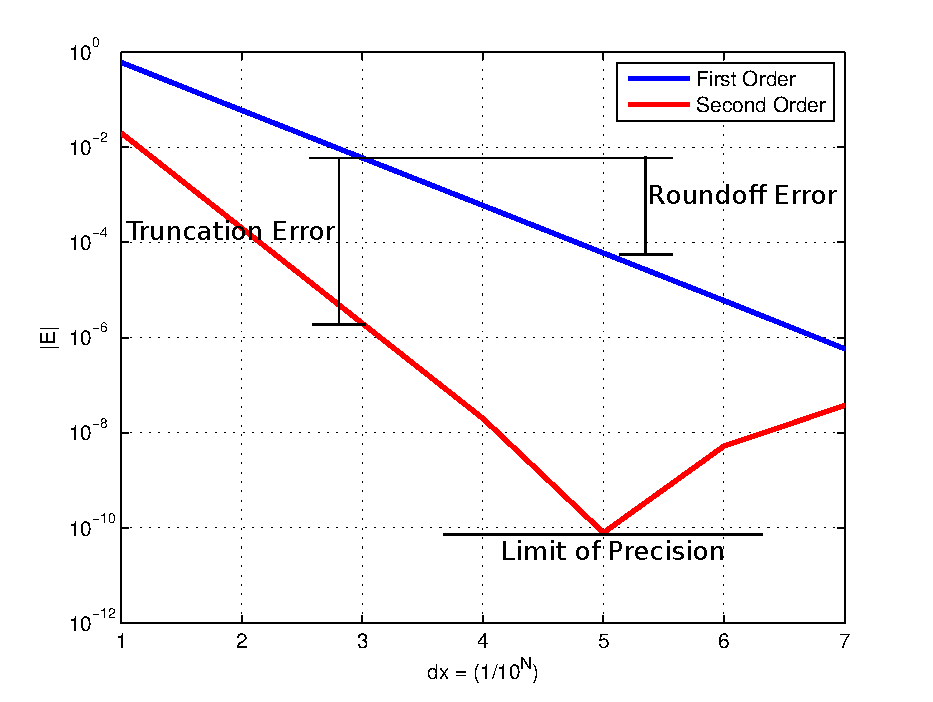
\includegraphics[height=0.55\textwidth,width=0.7\textwidth]{Graphics/Round_Off_Truncation.pdf}
      \end{center}
    \end{figure}
    
    Notice here that we can directly see that increasing our timestep
    reduces our round-off error. We can reduce our truncation error by
    using a higher and higher order method however we will always hit
    our limit of precision.

  \item {\bf Bicycle Sensor}

    Let's say I'd like to know my speed and distance while riding a
    bike. The easiest thing to do would be to install a sensor on the
    fork and the tire. When the sensor on the fork is in sync the main
    controller saves the time this happens in the form

    \begin{equation}
      T_{sync} = [T_1 \hdots T_N] 
    \end{equation}

    The task is then to extract velocity and distance from this
    equation. The first order derivative of velocity can be written in
    the form
    
    \beq
    V_i = \frac{x_{i+1} - x_i}{T_{i+1}-T_i} = \frac{\Delta x}{T_{i+1}-T_i}
    \eeq

    The question is what is $\Delta x$? $\Delta x$ is the distance the
    wheel travels during one click which is simply the circumference
    of the tire so we arrive at the equation below.

    \beq
    V_i = \frac{2\pi r}{T_{i+1}-T_i}
    \eeq

    To obtain the distance travelled we can apply the standard
    Reimmann Sum to the velocity equation above we obtain

    \beq
    x_N = x_0 + \sum\limits_{i=0}^N V_i \Delta T_i = \sum\limits_{i=0}^N
    \frac{2\pi r}{T_{i+1}-T_i}\Delta T_i = \sum\limits_{i=0}^N 2\pi r
    \eeq
  
    where $N$ is the number of times the sensor passes the main
    fork. Notice now that the sum does not depend on $i$ thus the
    distance is simply

    \beq
    x_N = x_0 + N2\pi r
    \eeq

    Which means we now have a method to determine velocity and
    distance traveled. As an example, try and verify the velocity and
    distance travelled using the timestamps below. Assume you're
    riding 14 inch tires.

    \beq
    \begin{matrix}
    T = [0,1.1320,4.1921,6.4561,8.3252,10.0598]~sec\\
    V = [6.4758,2.3955,3.2377,3.9219,4.2260]~ft/s\\
    X = [0,7.3304,14.6608,21.9911,29.3215,36.6519]~ft
    \end{matrix}
    \eeq

    \item {\bf Problems with Derivatives}
      
      Let's say I have a GPS sensor on an airplane traveling 800
      ft/s. This GPS sensor gives me two measurements. First the
      position in feet (Not really but we can just assume this for
      classroom example purposes).

      \beq
      X = [x_1 \hdots x_N] 
      \eeq

      The GPS is also timestamped and thus returns the time coordinate

      \beq
      T = [t_1 \hdots t_N]
      \eeq

      This seems like a simple problem. Just differentiate it and get

      \beq
      V_i = \frac{x_{i+1}-x_i}{t_{i+1}-t_{i}}
      \eeq

      The problem is real sensors have noise. So I can't actually know
      what $X$ is really and instead I obtain $\hat{X}$ which is my
      sampled measurement or output from the GPS sensor. Let's assume
      that my GPS is accurate to 25 ft. I can model this as:

      \beq\label{e:sampledX}
      \hat{X} = X + N(0,25)
      \eeq
      
      where $N(0,25)$ is a random uniform number with a mean of zero
      and a standard deviation of 25 ft. If we return to our numerical
      derivative we obtain

      \beq
      \hat{V}_i = \frac{\hat{x}_{i+1}-\hat{x}_i}{t_{i+1}-t_{i}}
      \eeq

      Ok so how bad is this? Let's compute the error between $V_i$ and
      $\hat{V}_i$.
      
      \beq
      V_i - \hat{V}_i =
      \frac{\hat{x}_{i+1}-\hat{x}_i}{t_{i+1}-t_{i}} -
      \frac{{x}_{i+1}-{x}_i}{t_{i+1}-t_{i}} = \frac{\hat{x}_{i+1}-\hat{x}_i -
        {x}_{i+1} + {x}_i}{t_{i+1}-t_{i}}
      \eeq

      If we substitute in equation \ref{e:sampledX} we obtain

      \beq
      V_i - \hat{V}_i =
      \frac{{x}_{i+1}+N_{i+1}-{x}_i-N_{i}-{x}_{i+1} +
        {x}_i}{t_{i+1}-t_{i}} = \frac{N_{i+1}-N_{i}}{t_{i+1}-t_{i}}
      \eeq

      Ok so let's substitute real number in here and obtain the
      maximum error remembering that GPS updates at 4 Hz = 0.25 sec

      \beq
      |V_i - \hat{V}_i|_{max} = \frac{|N_{i+1}-N_{i}|_{max}}{0.25 sec}
      \eeq

      So what is $|N_{i+1}-N_{i}|_{max}$. Well, the maximum of $N_i$
      is 25 ft which means that max of
      $|N_{i+1}-N_{i}|_{max}=25~ft$ which leads to 

      \beq
      |V_i - \hat{V}_i|_{max} = \frac{25~ft}{0.25~sec} = 100 ft/s
      \eeq

      Remember, we were flying at 800 ft/s and we could be off by as
      much as 100 ft/s! That's over 12.5\%. Notice however that, the
      velocity error is independent of flight speed so what would
      happen if we were riding a bike and our speed was say 10 ft/s?
      This would mean our velocity measurement was off by an order of
      magnitude. 
      
    \item {\bf Filters}

      We've shown in the previous derivation that derivatives
      introduce alot of noise in the measurement. So what do we do?
      The easiest thing to implement is what's called a complimentary
      filter. It is a simplification of the Kalman Filter created by
      Rudolf Kalman in 1960. The basic derivation goes like this,
      assume the input signal is $\hat{y}$ and the output filtered
      signal is $\tilde{y}$. This is the setup for all types of
      filters. In this setup we use the equation below

      \beq
      \tilde{y}_{i+1} = \sigma \hat{y}_{i+1} + (1-\sigma)\tilde{y}_{i}
      \eeq

      This may seem simple and it is but it's pretty
      powerful. Remember that the system is iterative so 

      \beq
      \begin{matrix}
        \tilde{y}_1 = \sigma \hat{y}_{1} + (1-\sigma)\tilde{y}_{0}\\
        \tilde{y}_2 = \sigma \hat{y}_{2} + (1-\sigma)\tilde{y}_{1}\\
        \tilde{y}_3 = \sigma \hat{y}_{3} + (1-\sigma)\tilde{y}_{2}\\
        \vdots\\
        \tilde{y}_N = \sigma \hat{y}_{N} + (1-\sigma)\tilde{y}_{N-1}
      \end{matrix}
      \eeq
      
      Notice that in this equation $\tilde{y}_0$ cannot be defined
      thus a separate equation is used for the initial condition. 

      \beq
      \tilde{y}_0 = \hat{y}_0
      \eeq

      With this setup we can now show some examples. Let's
      assume that $\sigma = 1$. In this scenario $\tilde{y}_i = \hat{y}_i$
      which means the signal is not filtered. If $\sigma = 0$,
      $\tilde{y}_{i+1} = \tilde{y}_i$. Since $\tilde{y}_0=\hat{y}_0$
      it means that that $\tilde{y}_i=\hat{y}_0$. However, if we
      return to the example where we have our GPS sensor on board and
      set $\sigma=0.03$ we obtain the following result. The other
      thing we can do of course is simply average the result. 

      \begin{figure}[H]
        \begin{center}
          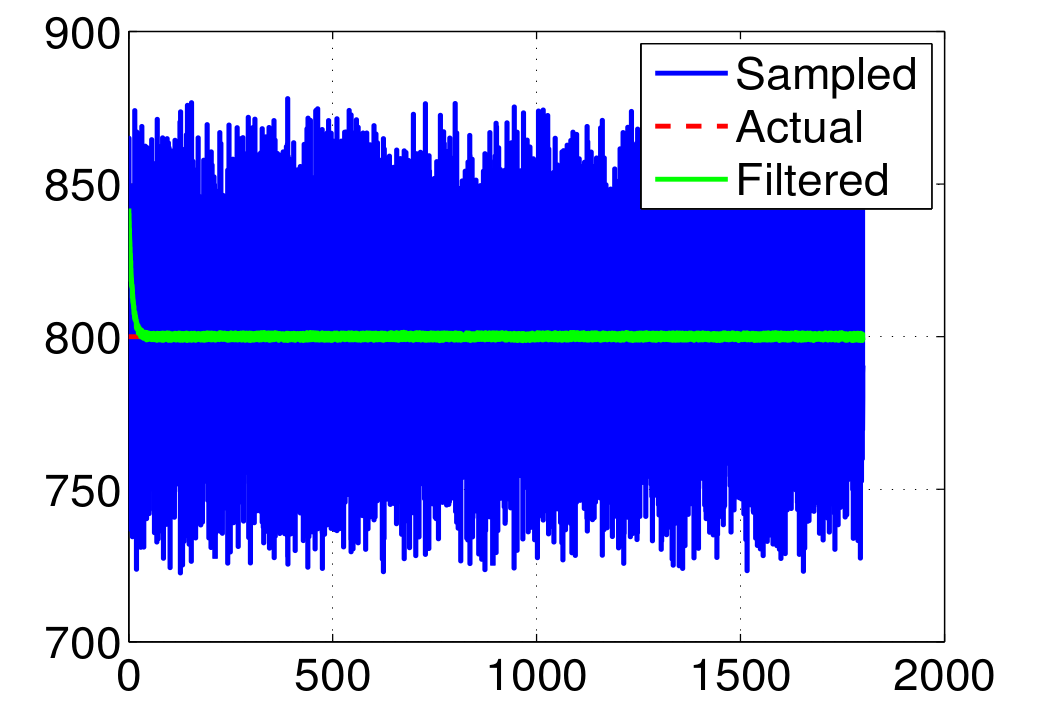
\includegraphics[height=0.5\textwidth,width=0.7\textwidth]{Graphics/Airplane_Sensor_Constant}
        \end{center}
      \end{figure}

      Now averaging the result would be easy when the speed is
      constant but airplanes rarely fly at constant speeds. What if
      the speed was more sinusoidal reflecting the changes in flight
      speed from atmospheric winds.

      \begin{figure}[H]
        \begin{center}
          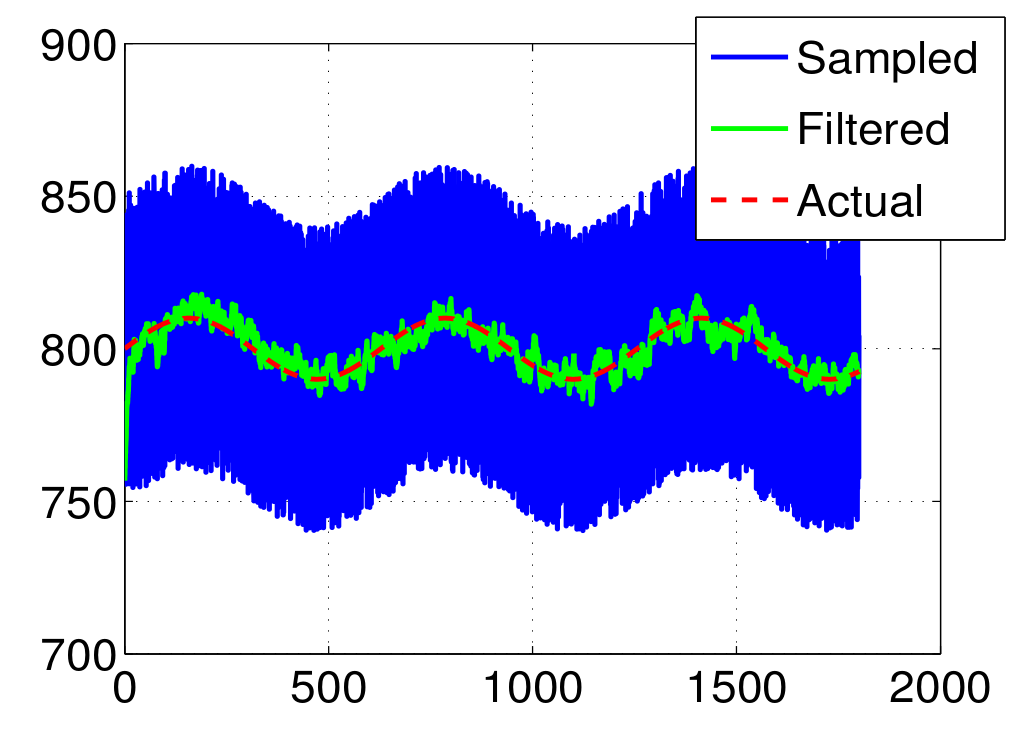
\includegraphics[height=0.5\textwidth,width=0.7\textwidth]{Graphics/Airplane_Sensor_Variable}
        \end{center}
      \end{figure}

      In the graph you can see that averaging the result does not
      simply capture the changes in the velocity of the airplane hence
      why the complimentary filter is so useful.
    
\end{enumerate}


